Our work spans over several areas such as altering the processor part of an \ac{sql} query engine and distributed transactions. There is also some work on high level interfaces for \acp{vlsd} that we find is worth mentioning.

\section{SQL over Memory}
The idea of patching Derby so that the data is stored in a different way than normal is not entirely new and was firstly introduced by Knut Magne Solem~\cite{derbyPatch}. In his approach all the tables whose name began with \emph{MEM} were stored in memory, as opposed to our approach which stores in Cassandra all the tables whose name starts with \emph{TUPLE}.

\section{Distributed Transactions}

Transactions become difficult under heavy load. When you first attempt to horizontally scale a relational database, making it distributed, you must now account for distributed transactions, where the transaction isn’t simply operating inside a single table or a single database, but is spread across multiple systems. In order to continue to honor the ACID properties of transactions, you need a transaction manager to orchestrate across the multiple nodes.

There are many leader election algorithms but they all have the same input and output. At the beginning there is a set of nodes in a network, unaware of which of them is the leader, after the protocol they all recognize a particular, unique node as the leader.

Assuming that the leader is already elected, a simple way to complete a distributed transaction in an atomic manner is for the coordinator to communicate the commit or abort request to all of the participants in the transaction and keep repeating the request until all of them have acknowledged that they have carried it out. This is called one-phase commit protocol~\cite{coulouris2005distributed} and is inadequate because it does not allow a server to make a unilateral decision to abort a transaction. 

\subsubsection{Two-phase commit protocol}

The two-phase commit protocol is designed to allow any participant to abort its part of a transaction which, by the atomicity requirement, means the whole transaction must be aborted. 

In the first phase of the protocol the coordinator asks all of the participants if they are prepared to commit and in the second it tells them to commit/abort the transaction. Once a participant has voted to commit a transaction it is not allowed to abort it, therefore a participant must before make sure it will be able to carry out its part of the protocol, before committing to it. 

\begin{table}[h!]
\centering
  \begin{tabular}{  l  p{8cm}}
	\toprule
	Operation & Description\\
    \midrule
    \emph{canCommit?(trans) $\rightarrow$ Yes/No} & Coordinator asks if it can commit a transaction. Participant replies with vote.\\  
    \emph{doCommit(trans)} & Coordinator tells participant to commit its part.\\
    \emph{doAbort(trans)} & Coordinator tells participant to abort its part.\\
    \emph{haveCommited(trans,participant)} & Participant tells the coordinator it has commited.\\
    \emph{getDecision(trans) $\rightarrow$ Yes/No} & Participant asks for decision after it has voted. Used to recover from server crashes or delayed messages.\\
	\bottomrule
  \end{tabular}

\caption{Operations for two-phase commit protocol (based on \cite{coulouris2005distributed})}
\label{tab:2pc_ops}
\end{table}

Using the operations defined in table \ref{tab:2pc_ops}, a successful run of the protocol with one coordinator and one participant is as shown by figure \ref{fig:2pc_run}.

\begin{figure}[htb]
  \begin{center}
    \leavevmode
    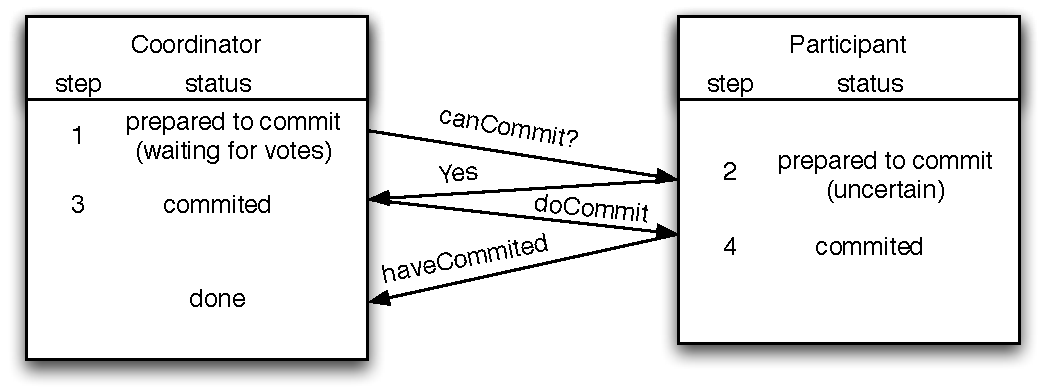
\includegraphics[width=0.9\textwidth]{images/2pc}
  \end{center}
  \caption{Two-phase commit successful run\cite{coulouris2005distributed}}
  \label{fig:2pc_run}
\end{figure}

\subsection{CloudTPS}
One particular implementation of distributed transactions, i.e. offers transactional guarantees (ACID) over a \ac{vlsd}, is CloudTPS~\cite{cloudTPS} which chooses to provide strong consistency at the cost of the possibility of becoming unavailable when facing network partition. In order to provide full transactional guarantees it introduces the concept of \acp{ltm} which are various parts of a transaction manager called transaction processing system, each of them is responsible for a part of the data and for processing certain parts of the transaction.

Since a transactional system must maintain the ACID properties even in the case of server failures, the data items and transactions state are replicated to multiple \acp{ltm} and consistent data snapshots are periodically checkpointed to the cloud storage system in order to guarantee the durability of each transaction.

The client can submit a transaction to any \ac{ltm} that is responsible for one of the accessed item, which then acts as the coordinator of the transaction across all \acp{ltm} responsible for the data items needed by the transaction, which is implemented using the two-phase commit protocol where the other \acp{ltm} are the participants.


\section{High Level Interfaces for a \ac{vlsd}}
\acp{vlsd}' query interfaces are in general very low level and do not conform to any type of standard which, as has been pointed out, leads to many problems including portability of code. There have been several projects that have proposed different high level interfaces for the \acp{vlsd} in order to mitigate this problem. 

\subsection{Object Mapper}

Using object mapping tools in order to allow to bypass the lower level interfaces of Cassandra is one the possible approaches, and is the one taken by the Cassandra Object Mapper~\cite{Pi}. 

In this project the user has at its disposal generic object interfaces like JPA and JDO that allow him to use the underlying database in an almost transparent way, which greatly simplifies the reading and writing of data. This transparency also brings the advantage of aiding in the migration of existent solutions and allowing the mix of different types of data stores under the same code base.  

The underlying store can be a Cassandra cluster which will, therefore, be available to the user through one of those interfaces with all their expressiveness and features, such as JDO class annotations.

One of the downsides of this solution is that it offer no transactional guarantees and therefore some of features that would be expected in this kind of the tool are thereby unavailable to the user. 

\subsection{Hive}
Hive~\cite{Thusoo:2009:HWS:1687553.1687609} was initially developed at Facebook and is now an Apache project. It is built on top of Apache Hadoop and facilitates querying and managing of large datasets in distributed storage by providing a mechanism to impose structure on a variety of data formats and access to files stored directly in Apache HDFS or in other storage systems. 

It defines a simple SQL-like query language, called \emph{HiveQL}, whose queries are executed via MapReduce with the particularity that there is no specific data format, it works on Thrift and allows for the creation of specialized data formats. Also, it enables users to plug in custom map-reduce scripts into queries.

Hive is not designed for online transaction processing and it is best used for batch jobs over large sets of append-only data since what it values most is scalability, extensibility, fault-tolerance and a loose coupling between it and its input formats. 

\subsection{\acl{cql}}

The \ac{cql} \cite{cql}, is a really novel approach to this matter, being developed by Eric Evans. His idea, is to develop a \ac{sql} like query language on top of Cassandra, bypassing an \ac{sql} interpreter altogether at the expense of not being compatible with actual \ac{sql}  code. Still, this would allow for much faster adaptation to Cassandra, for people with relational background. 

\ac{cql} has been released with Cassandra new stable version (0.8), and a select query will look somewhat like this \cite{cqlSelect}:

\begin{center}
\begin{verbatim}
    SELECT (FROM)? <CF> [USING CONSISTENCY.<LVL>] WHERE 
       <EXPRESSION> [ROWLIMIT X] [COLLIMIT Y] [ASC|DESC]
\end{verbatim}
\end{center}

And would be replacing a lot of old methods for retrieving data as \emph{get()}, \emph{get\_slice()}, \emph{get\_range\_slices()}, and so on.	

At the time of writing there are still some features to be implemented~\cite{cqlbbw}, such as \emph{ALTER} and prepared statements and some SQL features that will not be implemented at all, as joins and update\footnote{Since cassandra 0.7 the updates are viewed as a special case of insert}.
